\chapter{شناسایی و تحلیل ریسک‌ها}

شناسایی و تحلیل ریسک‌ها در سیستم حمل و نقل عمومی یک فرآیند حیاتی برای اطمینان از عملکرد بهینه و ایمن این سیستم است. این فرآیند به شناسایی، ارزیابی و اولویت‌بندی ریسک‌هایی می‌پردازد که می‌توانند بر عملکرد و ایمنی سیستم حمل و نقل تأثیر بگذارند. در ادامه، این فرآیند به طور مفصل تشریح می‌شود\cite{charnes1978}.

\section{شناسایی ریسک‌ها}
شناسایی ریسک‌ها اولین گام در تحلیل ریسک است و شامل شناسایی کلیه عواملی است که می‌توانند به هر نحوی عملکرد سیستم حمل و نقل عمومی را تحت تأثیر قرار دهند. این ریسک‌ها به دو دسته اصلی تقسیم می‌شوند: ریسک‌های داخلی و ریسک‌های محیطی.

\subsection{ریسک‌های داخلی}
\begin{enumerate}
	\item \textbf{مشکلات فنی و نگهداری}
	\begin{itemize}
		\item \textbf{خرابی وسایل نقلیه}: مشکلات مکانیکی یا الکتریکی در اتوبوس‌ها، متروها و قطارها که می‌تواند منجر به توقف یا تأخیر در خدمات شود. به عنوان مثال، خرابی موتور یا سیستم ترمز.
		\item \textbf{نگهداری نامناسب}: عدم انجام به‌موقع تعمیرات و نگهداری منظم که می‌تواند عمر مفید وسایل نقلیه را کاهش دهد و خطرات ایمنی ایجاد کند.
	\end{itemize}
	\item \textbf{مدیریت و منابع انسانی}
	\begin{itemize}
		\item \textbf{کمبود نیروی کار ماهر}: کمبود رانندگان و تکنسین‌های ماهر که می‌تواند به کاهش کیفیت خدمات و افزایش خطرات ایمنی منجر شود.
		\item \textbf{آموزش ناکافی کارکنان}: عدم ارائه آموزش‌های کافی به کارکنان در زمینه‌های ایمنی، خدمات مشتری و عملیات سیستم که می‌تواند کارایی را کاهش داده و خطرات را افزایش دهد.
	\end{itemize}
	\item \textbf{کارایی عملیاتی}
	\begin{itemize}
		\item \textbf{برنامه‌ریزی ناکارآمد مسیرها}: برنامه‌ریزی نامناسب مسیرها و زمان‌بندی‌ها که می‌تواند به تأخیرها، ازدحام و نارضایتی مسافران منجر شود.
		\item \textbf{ظرفیت ناکافی}: ناتوانی در پاسخ به تقاضای مسافران در ساعات اوج که می‌تواند به ازدحام و نارضایتی مسافران منجر شود.
	\end{itemize}
	\item \textbf{امنیت}
	\begin{itemize}
		\item \textbf{جرم و جنایت}: وقوع جرم و جنایت در ایستگاه‌ها و وسایل نقلیه که می‌تواند به کاهش احساس امنیت و نارضایتی مسافران منجر شود.
		\item \textbf{عدم آمادگی برای حوادث اضطراری}: ناتوانی در پاسخ به حوادث اضطراری مانند آتش‌سوزی یا حملات تروریستی که می‌تواند به خطرات جانی و مالی جدی منجر شود.
	\end{itemize}
\end{enumerate}

\subsection{ریسک‌های محیطی}
\begin{enumerate}
	\item \textbf{عوامل اقتصادی}
	\begin{itemize}
		\item \textbf{نوسانات قیمت سوخت}: تغییرات در قیمت سوخت که می‌تواند به افزایش هزینه‌های عملیاتی منجر شود.
		\item \textbf{وضعیت اقتصادی کلان}: رکود اقتصادی که می‌تواند به کاهش بودجه‌های دولتی و کاهش تقاضای حمل و نقل عمومی منجر شود.
	\end{itemize}
	\item \textbf{عوامل اجتماعی}
	\begin{itemize}
		\item \textbf{تغییرات جمعیتی}: تغییرات در جمعیت و توزیع جغرافیایی مسافران که می‌تواند به تغییر در تقاضا برای خدمات حمل و نقل منجر شود.
		\item \textbf{تغییر در الگوهای سفر}: تغییر در الگوهای کاری و زندگی که می‌تواند به تغییر در نیازهای حمل و نقل عمومی منجر شود.
	\end{itemize}
	\item \textbf{عوامل سیاسی و قانونی}
	\begin{itemize}
		\item \textbf{تغییرات در سیاست‌های دولتی}: تغییر در قوانین و مقررات که می‌تواند به تأثیرات مالی و عملیاتی برای سیستم حمل و نقل منجر شود.
		\item \textbf{نوسانات در حمایت‌های دولتی}: تغییرات در میزان و نوع حمایت‌های دولتی که می‌تواند به تغییر در بودجه‌ها و منابع مالی منجر شود.
	\end{itemize}
	\item \textbf{عوامل طبیعی و محیطی}
	\begin{itemize}
		\item \textbf{شرایط آب و هوایی نامناسب}: شرایط آب و هوایی شدید مانند برف، باران شدید یا طوفان که می‌تواند به تأخیرها و لغو خدمات منجر شود.
		\item \textbf{بلایای طبیعی}: وقوع بلایای طبیعی مانند زلزله، سیل یا آتش‌سوزی که می‌تواند به خرابی زیرساخت‌ها و وسایل نقلیه منجر شود.
	\end{itemize}
\end{enumerate}


\section{تجزیه و تحلیل درخت خطا (FTA) در سیستم حمل و نقل عمومی}

درخت خطا (\lr{Fault Tree Analysis}) یک روش گرافیکی و سیستماتیک برای تحلیل عوامل و رویدادهایی است که می‌توانند منجر به وقوع یک حادثه یا خرابی خاص در یک سیستم شوند. در تحلیل درخت خطا، رویدادهای ابتدایی (\lr{Basic Events}) که می‌توانند به یک رویداد اصلی (\lr{Top Event}) منجر شوند، شناسایی و تحلیل می‌شوند. این روش به شناسایی نقاط ضعف سیستم و تعیین راهکارهای پیشگیرانه کمک می‌کند.

\subsection{ساختار درخت خطا}

ساختار درخت خطا شامل یک نمودار درختی است که مسیرهای مختلفی را که می‌توانند منجر به وقوع یک حادثه خاص شوند، نشان می‌دهد. این نمودار از رویدادهای ابتدایی به سمت رویداد اصلی هدایت می‌شود. در ادامه، مراحل ساختار درخت خطا برای سیستم حمل و نقل عمومی را توضیح می‌دهیم.

\subsubsection{شناسایی رویداد اصلی}

رویداد اصلی (\lr{Top Event}) در تحلیل درخت خطا، حادثه یا خرابی اصلی است که می‌خواهیم از وقوع آن جلوگیری کنیم. در سیستم حمل و نقل عمومی، رویداد اصلی می‌تواند "توقف کامل سیستم حمل و نقل" باشد.

\subsubsection{شناسایی رویدادهای ابتدایی}

رویدادهای ابتدایی (\lr{Basic Events}) رویدادهایی هستند که به وقوع رویداد اصلی منجر می‌شوند. این رویدادها می‌توانند شامل عوامل فنی، مدیریتی، انسانی و محیطی باشند. برخی از رویدادهای ابتدایی در سیستم حمل و نقل عمومی عبارتند از:

\begin{itemize}
	\item خرابی وسایل نقلیه ($ V_1 $)
	\item نگهداری نامناسب ($ V_2 $)
	\item کمبود نیروی کار ماهر ($ H_1 $)
	\item آموزش ناکافی کارکنان ($ H_2 $)
	\item برنامه‌ریزی ناکارآمد مسیرها ($ O_1 $)
	\item شرایط آب و هوایی نامناسب ($ E_1 $)
\end{itemize}

\subsubsection{نمودار درخت خطا}

نمودار درخت خطا برای رویداد اصلی "توقف کامل سیستم حمل و نقل عمومی" به صورت زیر ترسیم می‌شود.
\begin{figure}[!ht]
	\centering
	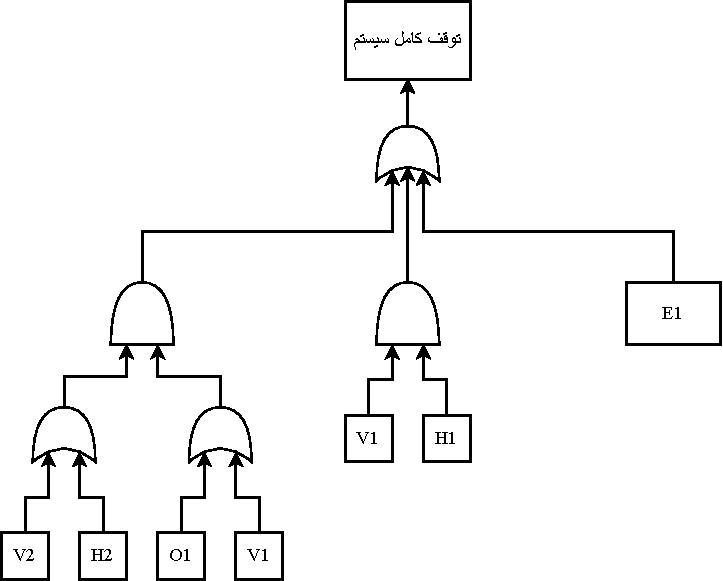
\includegraphics[width=0.5\linewidth]{fig/fig1.pdf}
	\caption{درخت خطای مربوط به سیستم حمل و نقل عمومی}
\end{figure}

\section{مدلسازی ریاضی}
با توجه به درخت خطا، مدل ریاضی به صورت زیر به دست می‌آید،
\begin{equation}
	1 - \left[1-\left[1-\left(1-X_1\right)\left(1-X_2\right)\right] \left[1-\left(1-X_3\right)\left(1-X_4\right)\right]\right] \left[1-X_4X_5\right] \left[1-X_6\right],
\end{equation}
که متغیرهای موجود در این عبارت ریاضی به صورت زیر نعریف شده‌اند،
\begin{itemize}
	\item $X_1$: نگهداری نامناسب
	\item $X_2$: آموزش ناکافی کارکنان
	\item $X_3$: برنامه‌ریزی ناکارآمد مسیرها
	\item $X_4$: خرابی وسایل نقلیه
	\item $X_5$: کمبود نیروی کار ماهر
	\item $X_6$: شرایط آب ‌و هوایی نامناسب
\end{itemize}